\documentclass{assignment}
\ProjectInfos{高等热力学与统计物理}{PHYS2110}{2020-2021学年第二学期}{习题 XI}{截止时间:2021. 5. 11(周二)}{陈稼霖}{45875852}

\begin{document}
\begin{prob}
    考虑临近作用的铁磁性 Ising 模型,写出自由能
    \[
        F_I(M)=-\frac{kT}{\mathcal{N}}\ln Q_{N_{\uparrow}}
    \]
    在零磁场下展开到 $M^4$ 的形式. 讨论此展开式在 $T>T_c$ 和 $T<T_c$ 的图像并求出两种情况下 $F_I(M)$ 的最小值和相应的磁化强度 $M$. (此类展开只适用于临界温度附近,故展开式中各项的系数只需保留到 $\abs{T-T_c}$ 的领头阶.)
\end{prob}
\begin{sol}
    Ising 模型的自由能为
    \begin{align}
        F_I(M)=-kT\ln Q_{N_{\uparrow}}=-\mu H\mathcal{N}M+\frac{n\varepsilon\mathcal{N}M^2}{2}+\frac{kT\mathcal{N}(1+M)}{2}\ln\frac{1+M}{2}+\frac{kT\mathcal{N}(1-M)}{2}\ln\frac{1-M}{2},
    \end{align}
    将其展开到 $M^4$ 的形式得
    \begin{align}
        \notag F_I(M)=&-\mu H\mathcal{N}M+\frac{n\varepsilon\mathcal{N}M^2}{2}+\frac{kT\mathcal{N}}{2}(1+M)\left[-\ln 2+M-\frac{1}{2}M^2+\frac{1}{3}M^3-\frac{1}{4}M^4\right]\\
        \notag&+\frac{kT\mathcal{N}}{2}(1-M)\left[-\ln 2-M-\frac{1}{2}M^2-\frac{1}{3}M^3-\frac{1}{4}M^4\right]\\
        =&\mathcal{N}kT\left[\frac{1}{12}M^4+\left(\frac{n\varepsilon}{2kT}+\frac{1}{2}\right)M^2-\frac{\mu H}{kT}M-\ln 2\right],
    \end{align}
    零磁场下,上式可化为
    \begin{align}
        F_I(M)=\mathcal{N}kT\left[\frac{1}{12}M^4+\left(\frac{n\varepsilon}{2kT}+\frac{1}{2}\right)M^2-\ln 2\right].
    \end{align}
    Bragg-Williams 公式:
    \begin{gather}
        \frac{\partial}{\partial M}\left(\frac{1}{\mathcal{N}}\ln Q_{N_{\uparrow}}\right)=0,\\
        \Longrightarrow \frac{1}{3}M^3=\left(\frac{T_c}{T}-1\right)M,
    \end{gather}
    其中 $T_c=-\frac{n\varepsilon}{k}$.

    当 $T>T_c$,$\frac{T_c}{T}+1>0$,由 Bragg-Williams 公式解得 $M=0$(图 \eqref{A11-P1-paramagnetic-phase}),亦即 $F_I(M)$ 仅有一个最小值,这一最小自由能为
    \begin{align}
        F_I(M=0)=-\mathcal{N}kT\ln 2.
    \end{align}
    \begin{figure}[H]
        \centering
        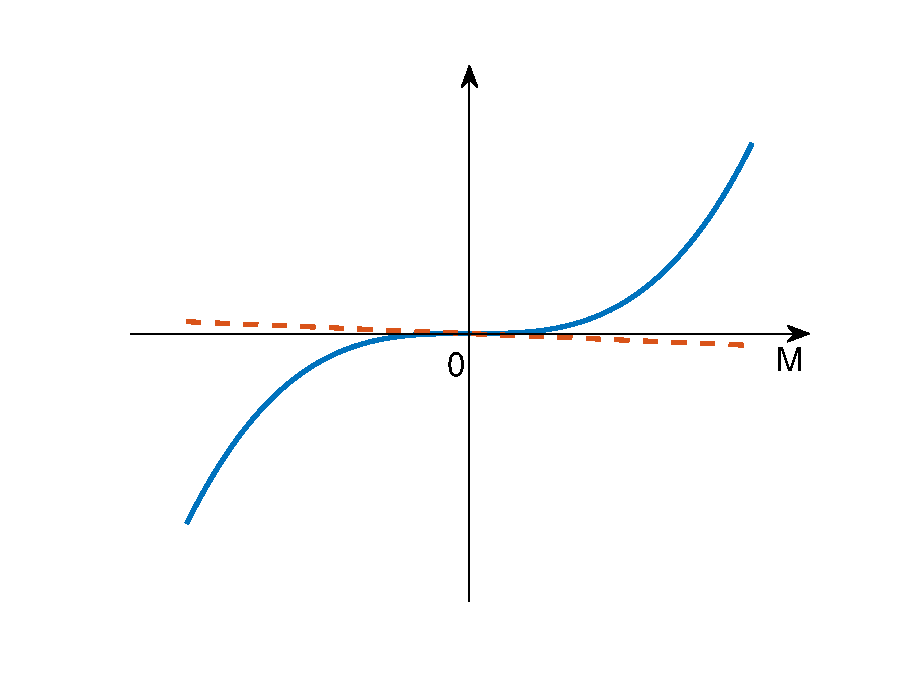
\includegraphics[width=.4\columnwidth]{A11-P1-paramagnetic-phase.eps}
        \caption{$T>T_c$ 下,Bragg-Williams 公式的情况,其中蓝线代表函数 $\frac{M^3}{3}$,橙线代表函数 $\left(\frac{T_c}{T}-1\right)M$}
        \label{A11-P1-paramagnetic-phase}
    \end{figure}

    当 $T<T_c$,$\frac{T_c}{T}+1<0$,由 Bragg-Williams 公式解得三个根 $M=0$, $M=\pm\sqrt{3\left(\frac{T_c}{T}-1\right)}$(图 \eqref{A11-P1-feromagnetic-phase}),其中
    \begin{align}
        \frac{\partial^2}{\partial M^2}F_I=\mathcal{N}kT\left(M^2+1-\frac{T_c}{T}\right)=\left\{\begin{array}{ll}
            \mathcal{N}kT\left(1-\frac{T_c}{T}\right)<0,&M=0,\\
            \frac{2}{3}\left(\frac{T_c}{T}-1\right)>0,&M=\pm\sqrt{3\left(\frac{T_c}{T}-1\right)}.
        \end{array}\right.
    \end{align}
    故 $F_I$ 在 $M=0$ 处取极大值,在 $M=\pm\sqrt{3\left(\frac{T_c}{T}-1\right)}$ 处取极小值. 自由能取极小值处即对应 Ising 的真实状态,此时自由能为
    \begin{align}
        F_I\left(M=\pm\sqrt{3\left(\frac{T_c}{T}-1\right)}\right)=\mathcal{N}kT\left[-\frac{17}{108}\left(\frac{T_c}{T}-1\right)^2-\ln 2\right].
    \end{align}
    \begin{figure}[H]
        \centering
        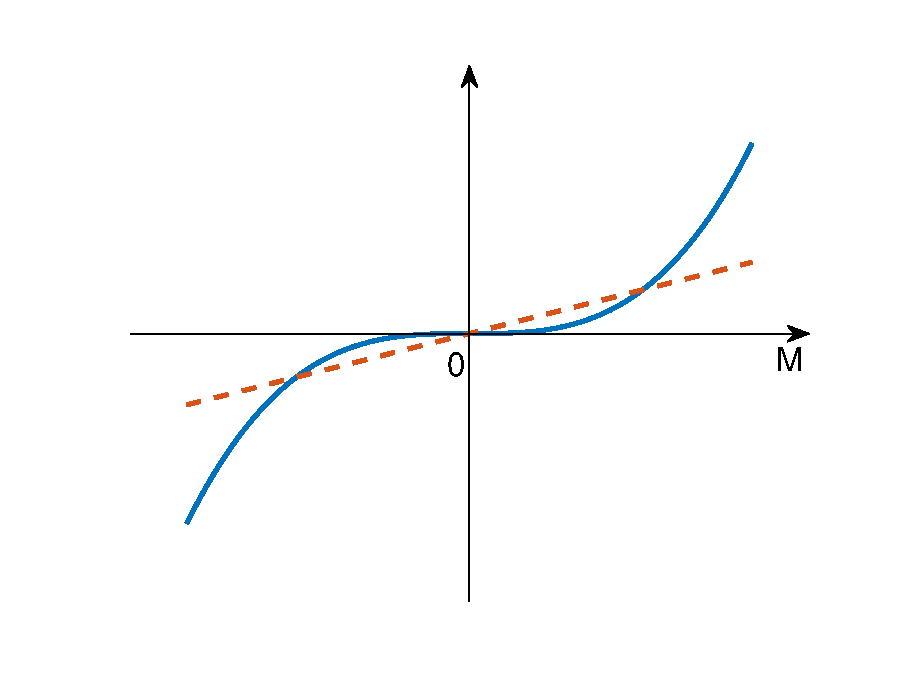
\includegraphics[width=.4\columnwidth]{A11-P1-feromagnetic-phase.eps}
        \caption{$T<T_c$ 下,Bragg-Williams 公式的情况,其中蓝线代表函数 $\frac{M^3}{3}$,橙线代表函数 $\left(\frac{T_c}{T}-1\right)M$}
    \end{figure}
\end{sol}
\end{document}